\documentclass[11pt]{book} % use larger type; default would be 10pt

\usepackage{ctex}
\usepackage{minted}

%%% Examples of Article customizations
% These packages are optional, depending whether you want the features they provide.
% See the LaTeX Companion or other references for full information.

%%% PAGE DIMENSIONS
\usepackage{geometry} % to change the page dimensions
\geometry{a4paper} % or letterpaper (US) or a5paper or....
% \geometry{margin=2in} % for example, change the margins to 2 inches all round
% \geometry{landscape} % set up the page for landscape
%   read geometry.pdf for detailed page layout information

\usepackage{graphicx} % support the \includegraphics command and options

% \usepackage[parfill]{parskip} % Activate to begin paragraphs with an empty line rather than an indent

%%% PACKAGES
\usepackage{booktabs} % for much better looking tables
\usepackage{array} % for better arrays (eg matrices) in maths
\usepackage{paralist} % very flexible & customisable lists (eg. enumerate/itemize, etc.)
\usepackage{verbatim} % adds environment for commenting out blocks of text & for better verbatim
\usepackage{subfig} % make it possible to include more than one captioned figure/table in a single float
% These packages are all incorporated in the memoir class to one degree or another...

%%% HEADERS & FOOTERS
\usepackage{fancyhdr} % This should be set AFTER setting up the page geometry
\pagestyle{fancy} % options: empty , plain , fancy
\renewcommand{\headrulewidth}{0pt} % customise the layout...
\lhead{}\chead{}\rhead{}
\lfoot{}\cfoot{\thepage}\rfoot{}

%%% SECTION TITLE APPEARANCE
\usepackage{sectsty}
\allsectionsfont{\sffamily\mdseries\upshape} % (See the fntguide.pdf for font help)
% (This matches ConTeXt defaults)

%%% ToC (table of contents) APPEARANCE
\usepackage[nottoc,notlof,notlot]{tocbibind} % Put the bibliography in the ToC
\usepackage[titles,subfigure]{tocloft} % Alter the style of the Table of Contents
\renewcommand{\cftsecfont}{\rmfamily\mdseries\upshape}
\renewcommand{\cftsecpagefont}{\rmfamily\mdseries\upshape} % No bold!

\usepackage{hyperref}

%%% END Article customizations

%%% The "real" document content comes below...

\title{机器学习基础知识}
\author{张洋}
%\date{} % Activate to display a given date or no date (if empty),
         % otherwise the current date is printed 

\begin{document}
\maketitle
\tableofcontents

\part{TensorFlow}

\chapter{TensorFlow 如何入门}

\section{第一部分}

\subsection{引言}

我们要解决的是一个过于简单且不现实的问题,但其好的一面是便于我们了解机器学习和 TensorFlow 的概念。我们要预测一个基于单一特征(房间面积/平方米)的单标量输出(房价/美元)。这样做消除了处理多维数据的需要,使我们能够在 TensorFlow 中只专注于确定、实现以及训练模型。

我们从一组收集到的数据点开始(见图 \ref{fig_tensorflow_sample_data}),每个数据点代表两个值之间的关系——输出(房价)与影响因素(房子面积)。

\begin{figure}
\centering
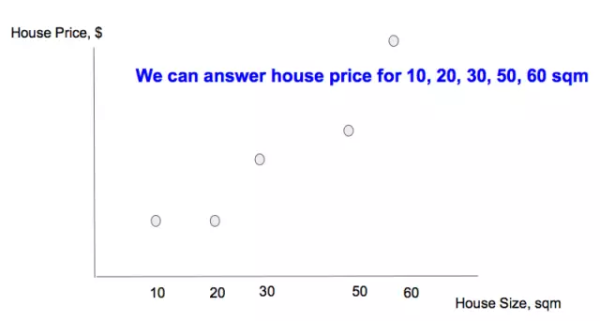
\includegraphics[width=\linewidth]{figures/tensorflow_sample_data}
\caption{}
\label{fig_tensorflow_sample_data}
\end{figure}

然而我们无法预测没有数据点的特征的值(见图 \ref{fig_tensorflow_sample_data_question})。

\begin{figure}
\centering
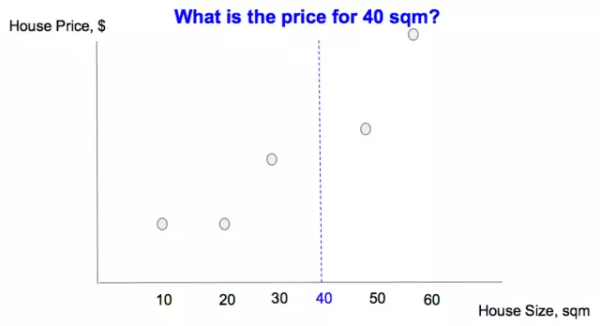
\includegraphics[width=\linewidth]{figures/tensorflow_sample_data_question}
\caption{}
\label{fig_tensorflow_sample_data_question}
\end{figure}

我们可以使用机器学习来挖掘它们之间的关系(见下图的「最佳拟合预测曲线」),即给定一个不属于数据点的特征值,我们可以准确地预测出输出(特征值和预测线的交点)。

\begin{figure}
\centering
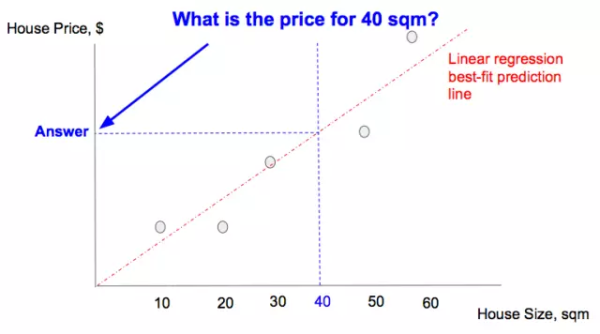
\includegraphics[width=0.7\linewidth]{figures/best_fit_prediction_line}
\caption{}
\label{fig:bestfitpredictionline}
\end{figure}


\subsection{步骤一:选择一个模型}

\subsubsection{1.模型种类}

为了使用机器学习来做预测,我们需要选择一个能够拟合收集到的数据的最佳模型。

我们可以选择一个线性(直线)模型,并通过改变其陡度/梯度和位置对其进行调整,从而匹配数据点。

\begin{figure}
\centering
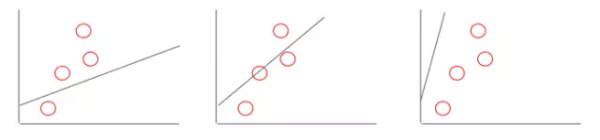
\includegraphics[width=0.7\linewidth]{figures/linear_model}
\caption{}
\label{fig:linearmodel}
\end{figure}


我们也可以选择一个指数(曲线)模型,并通过改变其曲率(curvature)和位置对其进行调整,从而匹配同一数据点集。

\begin{figure}
\centering
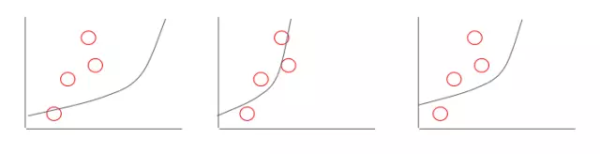
\includegraphics[width=0.7\linewidth]{figures/curve_model}
\caption{}
\label{fig:linearmodel}
\end{figure}

\subsubsection{2.成本函数}

为了比较哪个模型拟合得更严密,数学上我们将最佳拟合定义为一个需要被最小化的成本函数。 成本函数的一个简单样例是每个数据点所代表的实际输出与预测输出之间偏差的绝对值总和(实际结果到最佳拟合曲线的垂直投影)。用图表表示,成本函数被描述为下表中蓝色线段的长度和。

\begin{figure}
\centering
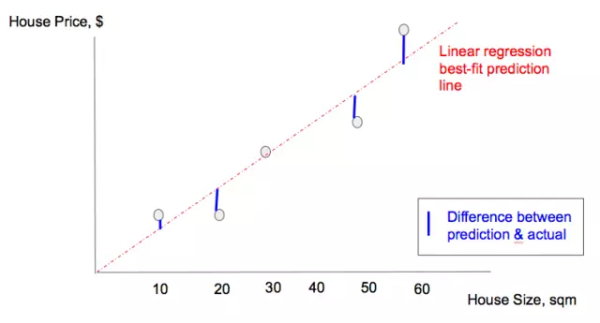
\includegraphics[width=0.7\linewidth]{figures/cost_function}
\caption{}
\label{fig:costfunction}
\end{figure}


注意:更准确地说,成本函数往往是实际输出和预测输出之间的方差,因为差值有时是负数;这也称为最小二乘法。

\subsubsection{3.线性模型简介}

秉持简洁精神,我们将使用线性模型来对数据点进行建模。线性模型的数学表示是:
  y= W.x + b
  Where:
  x: house size, in sqm
  y: predicted house price, in \$

为了调整模型来更好地拟合数据点,我们可以这样做:
调整 W 来改变线性模型的梯度

\begin{figure}
\centering
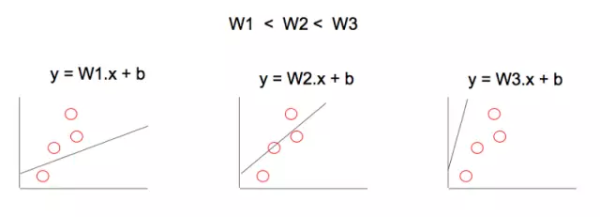
\includegraphics[width=0.7\linewidth]{figures/adjust_w}
\caption{}
\label{fig:adjustw}
\end{figure}


调整 b 来改变线性模型的位置

\begin{figure}
\centering
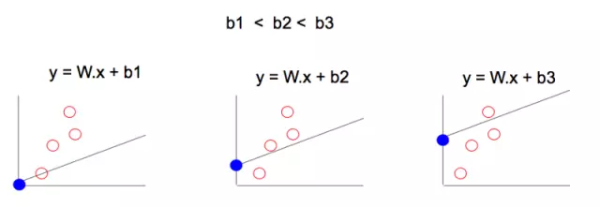
\includegraphics[width=0.7\linewidth]{figures/adjust_b}
\caption{}
\label{fig:adjustb}
\end{figure}


通过使用许多个 W、b 的值,最终我们可以找到一个最佳拟合线性模型,能够将成本函数降到最小。

除了随机尝试不同的值,有没有一个更好的方法来快速找到 W、b 的值?

\subsubsection{4.梯度下降}

如果你试图从山上下降到最低点,你的视角就是这个样子。

\begin{figure}
\centering
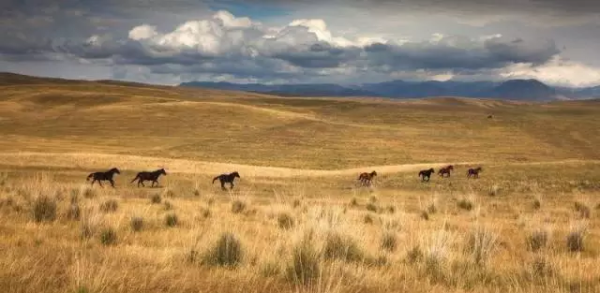
\includegraphics[width=0.7\linewidth]{figures/mountain}
\caption{}
\label{fig:mountain}
\end{figure}


下降趋势并不明显!其最佳方式是执行梯度下降:
\begin{enumerate}
    \item 在当前位置以最陡的下降梯度确定方向
    \item 在该方向上采取步长 X
    \item 重复 \& 刷新;这就是训练过程
\end{enumerate}

最小化成本函数是类似的,因为成本函数就像是起伏的山,我们想要找到其中的最低点,我们可以通过梯度下降类似地实现。

\begin{figure}
\centering
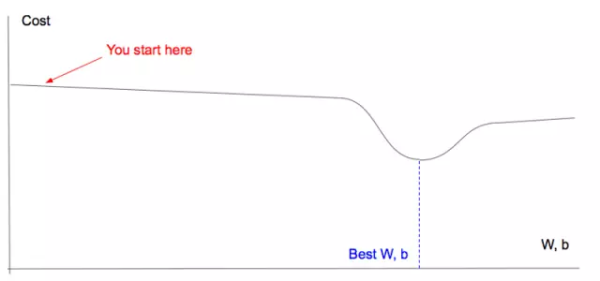
\includegraphics[width=0.7\linewidth]{figures/mountain_solution}
\caption{}
\label{fig:mountainsolution}
\end{figure}


现在我们有了线性模型、成本函数和梯度下降的概念,可以开始使用 TensorFlow 了。

\subsection{步骤二:在TensorFlow 中建立模型}

\subsubsection{1.TensorFlow 中的线性模型}

TensorFlow 的2个基本组件是:

\begin{enumerate}
    \item 占位符(Placeholder):表示执行梯度下降时将实际数据值输入到模型中的一个入口点。例如房子面积  (x) 和房价 (y\_)。
    
    \begin{minted}{python}
x = tf.placeholder(tf.float32, [None, 1])  
    \end{minted}
    
    \item 变量:表示我们试图寻找的能够使成本函数降到最小的「good」值的变量,例如 W 和 b。
    \begin{minted}{python}
W = tf.Variable(tf.zeros([1, 1]))
b = tf.Variable(tf.zeros([1]))
    \end{minted}
\end{enumerate}

然后 TensorFlow 中的线性模型$  (y = W.x + b)  $就是:

\begin{minted}{python}
y = tf.matmul(x, W) + b
\end{minted}


\subsubsection{2.TensorFlow 中的成本函数}
与将数据点的实际房价 (y\_) 输入模型类似,我们创建一个占位符。

\begin{minted}{python}
y_ = tf.placeholder(tf.float32, [None, 1])
\end{minted}

成本函数的最小方差就是:

\begin{minted}{python}
cost = tf.reduce_sum(tf.pow((y_ - y), 2))
\end{minted}

\subsubsection{3.数据}
由于没有房价(y\_) 和房子面积 (x) 的实际数据点,我们就生成它们。

\begin{minted}{python}
for i in range(100):
    //Create fake data for actual data
    xs = np.array([[i]])
    ys = np.array([[2 * i]])
\end{minted}

简单起见,我们将房价 (ys) 设置成永远是房子面积 (xs) 的 2 倍。

\subsubsection{4.梯度下降}
有了线性模型、成本函数和数据,我们就可以开始执行梯度下降从而最小化代价函数,以获得 W、b 的「good」值。

\begin{minted}{python}
train_step = tf.train.GradientDescentOptimizer(0.00001).minimize(cost)
\end{minted}

0.00001 是我们每次进行训练时在最陡的梯度方向上所采取的「步」长;它也被称作学习率(learning rate)。

\subsection{步骤三:训练模型}
训练包含以预先确定好的次数执行梯度下降,或者是直到成本函数低于某个预先确定的临界值为止。

\subsubsection{1.TensorFlow 的怪异}
所有变量都需要在训练开始时进行初始化,否则它们可能会带有之前执行过程中的残余值。

\begin{minted}{python}
init = tf.initialize_all_variables()
\end{minted}

\subsubsection{2.TensorFlow 会话}
虽然 TensorFlow 是一个 Python 库,Python 是一种解释性的语言,但是默认情况下不把 TensorFlow 运算用作解释性能的原因,因此不执行上面的 init 。相反 TensorFlow 是在一个会话中进行;创建一个会话 (sess) 然后使用 sess.run() 去执行。

\begin{minted}{python}
sess = tf.Session()
sess.run(init)
\end{minted}

类似地我们在一个循环中调用 withinsess.run() 来执行上面的 train\_step。

\begin{minted}{python}
for i in range(steps):
    //Create fake data for actual data
    xs = np.array([[i]])
    ys = np.array([[2 * i]])
    
    #Trainning
    feed = {x:xs, y_:ys}
    sess.run(train_step, feed_dict = feed)
    
    print("After %d iteration:" % i)
    print("W: %f" % sess.run(W))
    print("b: %f" % sess.run(b))
\end{minted}

你需要将由 x, y\_ 所组成的实际数据输入再提供给输入,因为 TensorFlow 将 train\_step 分解为它的从属项:

\begin{figure}
\centering
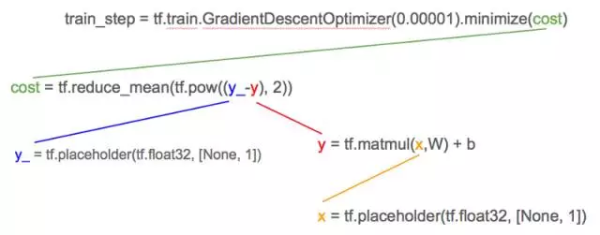
\includegraphics[width=0.7\linewidth]{figures/train_steps}
\caption{}
\label{fig:trainsteps}
\end{figure}


从属项的底部是占位符 x,y\_;而且正如我们之前提到的,tf.placeholders 是用来表示所要提供的实际数据点值房价 (y\_) 和房子面积  (x) 的位置。

\subsubsection{结果}
循环中的 print 语句将显示 TensorFlow 如何在每次迭代中学习 W 和 b 的「good」值。

\begin{figure}
\centering
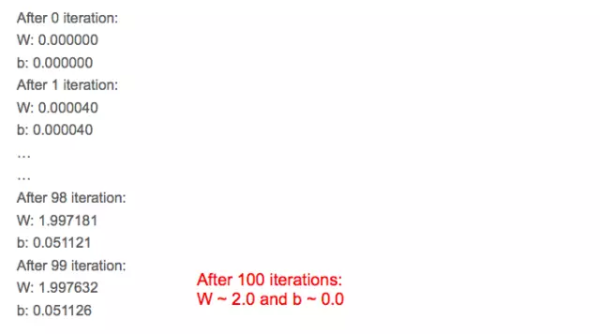
\includegraphics[width=0.7\linewidth]{figures/result}
\caption{}
\label{fig:result}
\end{figure}


\subsubsection{小结}
我们已经以最简单的形式学习了机器学习;从一个单一特征预测结果。(为简单起见)我们选择了一个线性模型来拟合我们的数据点,定义一个成本函数来表示最佳拟合,并通过反复调整其梯度变量 W 与位置变量 b 来训练我们的模型,使成本函数降到最小。

\section{第二部分}

简单回顾
在上一部分,我们使用 TensorFlow 构建并学习了一个带有单一特征的线性回归模型——给定一个特征值(房屋面积/平方米),我们可以预测输出(房价/美元)。

下面是一些总结:
\begin{enumerate}
    \item 我们有一些房屋面积和房价的数据(灰色点)
    \item 我们使用线性回归对这些数据进行了建模(红色虚线)
    \item 我们通过训练该线性回归模型的 W(权重)和 b(偏置)找到了最小化「成本」(竖直蓝色实线的长度总和,这些蓝线代表了预测和实际输出之间的差异)的「最好」模型
    \item 给定任意房屋面积,我们可以使用该线性模型预测房价(带箭头的蓝色虚线)
\end{enumerate}

一张图解释线性回归

\begin{figure}
\centering
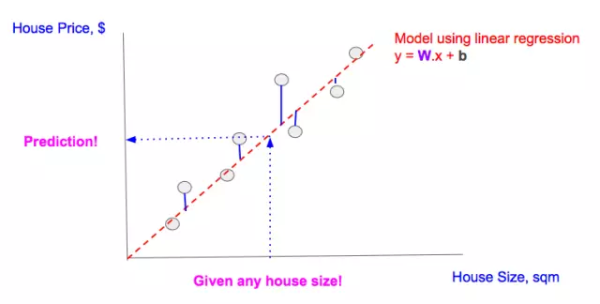
\includegraphics[width=0.7\linewidth]{figures/linear_regression}
\caption{}
\label{fig:linearregression}
\end{figure}


在机器学习文献中,我们常常看到「训练(training)」这个词。在这一部分,我们将在 TensorFlow 中理解「训练」的含义。

\subsection{线性回归建模}
Linear Model (in TF notation): y = tf.matmul(x,W) + b

线性回归的目标是寻找 W 和 b,这样对于给定的任意特征值 x,我们可以通过将 W、b 和 x 的值代入到模型中得到预测 y。

但是为了找到能准确做出预测的 W 和 b 的值,我们需要使用可用的数据(许多实际特征 x 和实际输出 y\_ 的配对,注意下划线)来「训练」该模型。

\subsection{解释「训练」}

为了找到最佳的 W 和 b 值,我们可以从任意的 W 和 b 值开始。我们也需要定义一个成本函数,该函数可以衡量对于一个给定特征值 x 预测输出 y 和实际输出 y\_ 之间差异。为了简单起见,我们使用最简单的最小均方误差(MSE:minimum squared error)作为我们的成本函数。
Cost function (in TF notation): tf.reduce\_mean(tf.square(y\_ - y))

通过最小化成本函数,我们可以得到很好的 W 和 b 值。

我们的训练代码实际上非常简单,并且用 [A, B, C, D]

 \url{https://github.com/nethsix/gentle_tensorflow/blob/master/code/linear_regression_one_feature_using_mini_batch_with_tensorboard.py}

\begin{minted}{python}
# ... (省略) 变量/常量声明 ...

# [A] TensorFlow图
y = tf.matmul(x,W) + b
cost = tf.reduce_mean(tf.square(y_-y))

# [B] 用固定「学习率(learn_rate)」训练
learn_rate = 0.1
train_step =
   tf.train.GradientDescentOptimizer(learn_rate).minimize(cost)

for i in range(steps):
 # [C] 准备数据点
 # ... (省略) 准备作为x和y的数据点的代码 ...

 # [D] 在每个步骤/epoch将数据送入'train_step'
 feed = { x: xs, y_: ys }
 sess.run(train_step, feed_dict=feed)
 \end{minted}

我们的线性模型和成本函数[A]可以表示成下面的 TensorFlow 图:

\begin{figure}
\centering
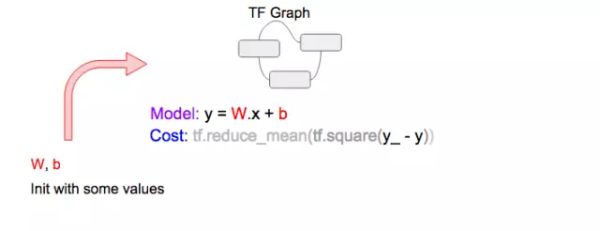
\includegraphics[width=0.7\linewidth]{figures/linear_cost}
\caption{}
\label{fig:linearcost}
\end{figure}


创造一个带有模型和成本函数的 TensorFlow 图,并使用一些值初始化 W 和 b

接下来,我们选择一个数据点 (x, y\_) [C],然后将其送入[D] TensorFlow 图,从而得到预测 y 和相应的成本。

\begin{figure}
\centering
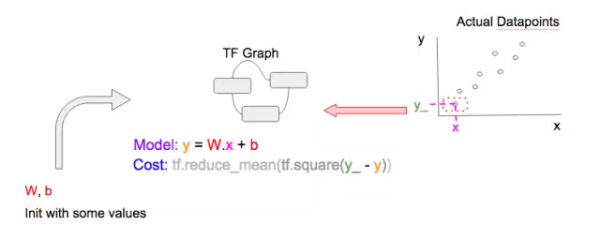
\includegraphics[width=0.7\linewidth]{figures/linear_prediction}
\caption{}
\label{fig:linearprediction}
\end{figure}


使用单个数据点计算预测 y 和成本

为了得到更好的 W 和 b,我们使用TensorFlow 的 tf.train.GradientDescentOptimizer [B]执行梯度下降以降低成本。用非技术的术语来说:给定当前成本,并基于成本岁其它变量(即 W 和 b)的变化方式,优化器(optimizer)将对 W 和 b 执行一些小调整(递增或递减)以使我们的预测更好地契合那个单个数据点。

\begin{figure}
\centering
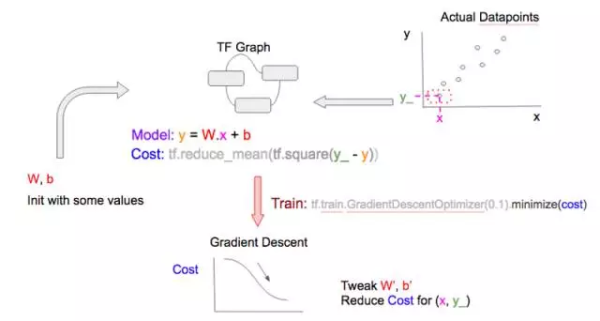
\includegraphics[width=0.7\linewidth]{figures/optimization}
\caption{}
\label{fig:optimization}
\end{figure}


基于当前的成本,决定如何调整 W 和 b 以提升预测 y 和降低成本

训练周期中的最后步骤是在调整 W 和 b 对它们进行更新。注意这里的「周期」用机器学习的术语来说是「epoch」。

\begin{figure}
\centering
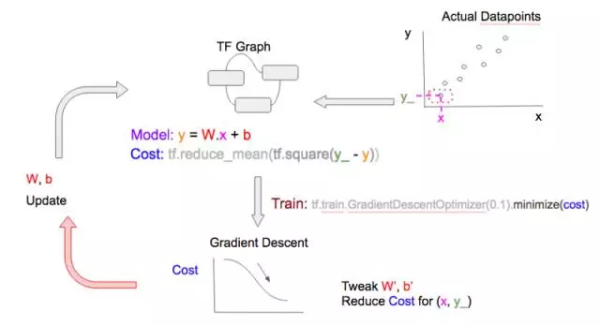
\includegraphics[width=0.7\linewidth]{figures/epoch}
\caption{}
\label{fig:epoch}
\end{figure}


在下一训练 epoch 的迭代前,通过调整 W 和 b 对它们进行更新

在下一训练 epoch 中,重复这些步骤,但使用一个不同的数据点!

\begin{figure}
\centering
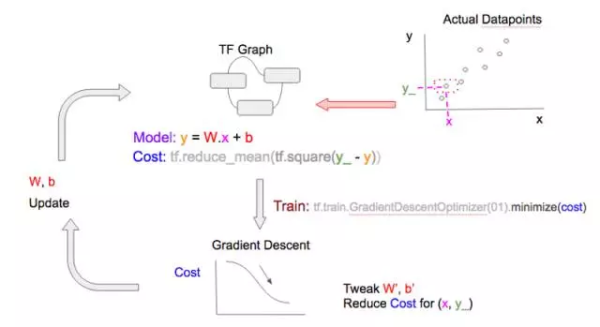
\includegraphics[width=0.7\linewidth]{figures/epoch_iter}
\caption{}
\label{fig:epochiter}
\end{figure}


使用不同的数据点进行训练

使用各种数据点泛化(generalize)我们的模型,即学习可被用于预测任何特征值的 W 和 b 值。注意:
\begin{enumerate}
    \item 在大部分情况下,数据点越多,模型的学习和泛化就越好
    \item 如果你训练的 epoch 比数据点还多,你可以重复使用数据点,这不成问题。梯度下降优化总是会同时使用数据点及其成本(根据该 epoch 的 W 和 b 值从数据点中计算得到)来对 W 和 b 值进行调整;该优化器也许之前已经见过了这个数据点,但成本并不一样,因此它还是可以学到新的东西,并以不同的方式调整 W 和 b 值。
\end{enumerate}

你可以用固定数量的 epoch 训练一个模型,直到其达到令人满意的成本阈值。

\subsection{训练变量}

\subsubsection{1.随机、mini-batch、batch}
在上面的训练中,我们在每个 epoch 送入单个数据点。这被称为随机梯度下降(stochastic gradient descent)。我们也可以在每个 epoch 送入一堆数据点,这被称为 mini-batch 梯度下降,或者甚至在一个 epoch 一次性送入所有的数据点,这被称为 batch 梯度下降。请看下图的比较,注意这 3 张图的 2 处不同:

\begin{enumerate}
\item 每个 epoch 送入 TensorFlow 图(TF.Graph)的数据点的数量(图右上方)
\item 梯度下降优化在调整 W 和 b 值时所考虑的数据点的数量(图右下方)
\end{enumerate}

随机梯度下降

\begin{figure}
\centering
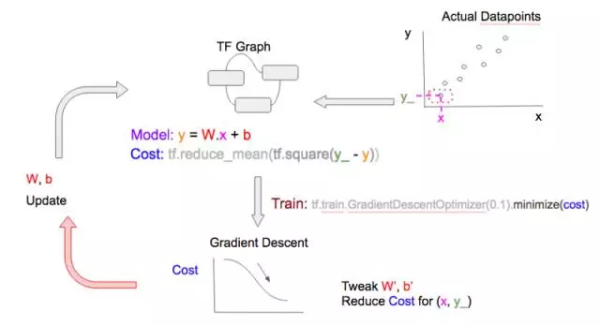
\includegraphics[width=0.7\linewidth]{figures/down}
\caption{}
\label{fig:down}
\end{figure}


mini-batch 梯度下降
\begin{figure}
\centering
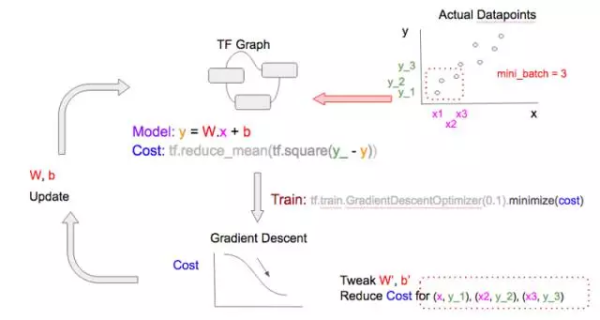
\includegraphics[width=0.7\linewidth]{figures/minibatch}
\caption{}
\label{fig:minibatch}
\end{figure}


batch 梯度下降
\begin{figure}
\centering
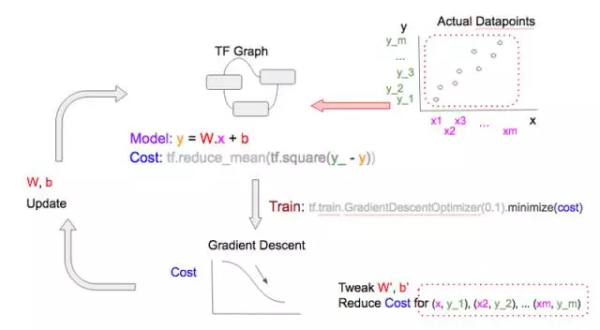
\includegraphics[width=0.7\linewidth]{figures/batch}
\caption{}
\label{fig:minibatch}
\end{figure}


每张图中的数据点的数量有 2 个含义。当数据点更多时:
\begin{enumerate}
\item 计算成本和执行梯度下降所需的计算资源(减法、平方、加法)会增加
\item 模型的学习和泛化的速度增加
\end{enumerate}

选择随机、mini-batch、batch 梯度下降的优缺点总结在下图中:

\begin{figure}
\centering
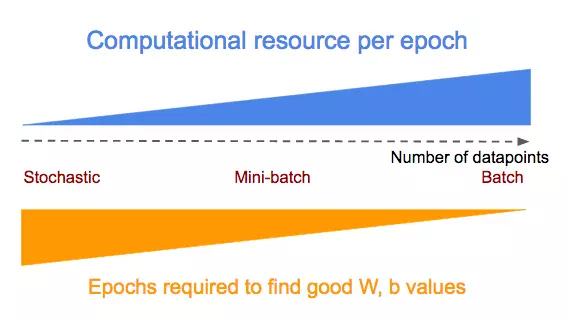
\includegraphics[width=0.7\linewidth]{figures/advantages}
\caption{}
\label{fig:advantages}
\end{figure}


选择随机、mini-batch、batch 梯度下降的优缺点

要在随机/mini-batch/batch 梯度下降之间切换,我们只需要在将数据点送入训练步骤[D]之前将这些数据点分成不同的 batch 大小,即为 [C] 使用如下的代码片段:

\begin{minted}{python}
# * all_xs: 所有的特征值
# * all_ys: 所有的输出值
# datapoint_size: all_xs/all_ys 中点/项的数量
# batch_size: 配置如下:
#             1: 随机模型
#             integer < datapoint_size: mini-batch模式
#             datapoint_size: batch模式
# i: 当前epoch数量

if datapoint_size == batch_size:
 # Batch 模式,所以选择所有数据点从 index 0 开始
 batch_start_idx = 0
elif datapoint_size < batch_size:
 # 不可能
 raise ValueError(“datapoint_size: %d, must be greater than         
                   batch_size: %d” % (datapoint_size, batch_size))
else:
 # 随机/mini-batch模式: 从所有可能的数据点中分批选择数据点
 batch_start_idx = (i * batch_size) % (datapoint_size — batch_size)
 batch_end_idx = batch_start_idx + batch_size
 batch_xs = all_xs[batch_start_idx:batch_end_idx]
 batch_ys = all_ys[batch_start_idx:batch_end_idx]

# 将分批的数据点定义为xs, ys, 它们会被送入 'train_step'训练步骤
xs = np.array(batch_xs)
ys = np.array(batch_ys)
\end{minted}

\subsubsection{2.学习率变化}

学习率(learn rate)是指梯度下降调整 W 和 b 递增或递减的速度。学习率较小时,处理过程会更慢,但肯定能得到更小成本;而当学习率更大时,我们可以更快地得到最小成本,但有「冲过头」的风险,导致我们没法找到最小成本。

为了克服这一问题,许多机器学习实践者选择开始时使用较大的学习率(假设开始时的成本离最小成本还很远),然后随每个 epoch 而逐渐降低学习率。

TensorFlow 提供了 2 http://stackoverflow.com/questions/33919948/how-to-set-adaptive-learning-rate-for-gradientdescentoptimizer;但这里进行了总结。

使用梯度下降优化的变体
TensorFlow 带有多种支持学习率变化的梯度下降优化器,例如  tf.train.AdagradientOptimizer 和 tf.train.AdamOptimizer.

使用 tf.placeholder 调整学习率
如同前面所看到的,如果我们在这个例子中声明了 tf.placeholder 来设置学习率,然后在 tf.train.GradientDescentOptimizer 中使用它,我们可以在每个训练 epoch 向其送入一个不同的值,这很像我们给 x 和 y\_ 送入不同的数据点,这也是每个 epoch 的 tf.placeholders.

我们需要 2 个小修改:
\begin{minted}{python}
# 修改 [B] ,将 'learn_rate' 设置为'tf.placeholder'
# 并将其提供给'learning_rate'参数名tf.train.GradientDescentOptimizer
learn_rate = tf.placeholder(tf.float32, shape=[])
train_step = tf.train.GradientDescentOptimizer(
   learning_rate=learn_rate).minimize(cost)

# 修改[D],包含送入一个'learn_rate'值,
# 即 'initial_learn_rate'(初始学习率)除以'i' (当前epoch数)
# 注: 这是过于简化的,仅用作示例
feed = { x: xs, y_: ys, learn_rate: initial_learn_rate/i }
sess.run(train_step, feed_dict=feed)
\end{minted}

\subsection{小结}
我们解释了机器学习中「训练(training)」的含义,以及在 TensorFlow 中通过模型和成本定义、然后循环通过训练步骤(将数据点送入梯度下降优化器)来进行训练的方式。我们还讨论了训练中的常见变量,即改变模型学习时每个 epoch 所用的数据点的大小和改变梯度下降优化器的学习率。

\section{第三部分:矩阵和多特征线性回归}
快速回顾
之前文章的前提是:给定特征——任何房屋面积(sqm),我们需要预测结果,也就是对应房价(\$)。为了做到这一点,我们:
我们找到一条「最拟合」所有数据点的直线(线性回归)。「最拟合」是当线性回归线确保实际数据点(灰色点)和预测值(内插在直线上的灰色点)之间的差异最小,即最小化多个蓝线之和。
使用这条直线,我们可以预测任何房屋的价格。

使用单一特征线性回归进行预测 

多特征线性回归概述
实际上,任何预测都依赖于多个特征,于是我们从单特征的线性回归进阶到 带有两个特征的线性回归;之所以选择两个特征,是为了让可视化和理解简明些,但这个思想可以推广到带有任何数量特征的线性回归。
我们引进一个新的特征——房间数量。当收集数据点时,现在我们需要在现有特征「房屋面积」之上收集新特征「房间数」的值,以及相应的结果「房屋价格」。

我们的图表变成了 3 维的。

结果「房屋价格」以及 2 个特征(「房间数」,「房屋面积」)的数据点空间 

然后,我们的目标变成:给定「房间数」和「房屋面积」,预测「房屋价格」(见下图)。

由于缺少数据点,有时无法对给定的 2 个特征进行预测 

在单一特征的情形中,当没有数据点时,我们需要使用线性回归来创建一条直线,以帮助我们预测结果房屋价格。在 2 个特征的情形中,我们也可以使用线性回归,但是需要创建一个平面(而不是直线),以帮助我们预测(见下图)。

使用线性回归在 2 个特征空间中的创建一个平面来做预测 

多特征线性回归模型
回忆单一特征的线性回归(见下图左边),线性回归模型结果为 y,权重为 W,房屋大面积为 x,偏差为 b。
对于 2 个特征的回归(参见下图右侧),我们引入另一个权重 W2,另一个自变量 x2 来代表房间数的特征值。


单特征 vs. 2 个特征的线性回归方程 

如之前讨论的那样,当我们执行线性回归时,梯度下降算法能帮助学习系数 W、W2 和 b 的值。

Tensorflow 的多特征线性回归
1.快速回顾
单特征线性回归的 TF 代码由 3 部分组成(见下图):
构建模型(蓝色部分)
基于模型构建成本函数(红色部分)
使用梯度下降(绿色部分)最小化成本函数

用于单特征线性回归的 Tensorflow 代码 

2.Tensorflow 的 2 个特征的线性回归
TF 代码中 2 个特征的线性回归方程(如上所述)的变化(相比单特征)用红色显示。

注意,增加新特征的这种方式效率低;随着特征数量的增长,所需的变量系数和自变量的数量会增加。实际的模型有更多的特征,这恶化了这个问题。那么,如何能有效地表示特征呢?

解决方法:矩阵
首先,让我们将表征两个特征的模型推广到表征 n 个特征的模型:


复杂的 n 特征公式可以用矩阵简化,矩阵被内置于 TF 中,这是因为:
数据可以用多维表示,这契合我们表征具有 n 个特征的数据点(左下方,也称为特征矩阵)以及具有 n 个权重模型(右下,也称为权重矩阵)的方式

单个数据点的 n 个特征与模型的矩阵形式的 n 个权重 

在 TF 中,它们将被写为:
x = tf.placeholder(tf.float,[1,n])
W = tf.Variable(tf.zeros [n,1])
注意:对于 W,我们使用 tf.zeros,它将所有 W1,W2,...,Wn 初始化为零。
在数学上,矩阵乘法是向量乘法的加总;因此自然地,特征(中间的一个)和权重(右边的)矩阵之间的矩阵乘法给出(左边的)结果,即等于 n 个特征的线性回归公式的第一部分(如上所述),没有截距项。


特征和权重矩阵之间的矩阵乘法给出结果(未添加截距项) 

在 TF 中,这种乘法将表示为:
y = tf.matmul(x, W)
多行特征矩阵(每行表示数据点的 n 个特征)之间的矩阵乘法返回多行结果,每行代表每个数据点的结果/预测(没有加入截距项);因此一个矩阵乘法就可以将线性回归公式应用于多个数据点,并对应地产生多个预测(每个数据点对应一个结果)(见下文)

注意:特征矩阵中的 x 表示变的更复杂,即我们使用 x1.1、x1.2,而不是 x1、x2 等,因为特征矩阵(中间矩阵)从表示 n 个特征(1 行 x,n 列)的单个数据点扩展到表示具有 n 个特征(m 行 x,n 列)的 m 个数据点。因此,我们扩展 x <n>(如 x1)到 x <m >.<n>(如 x1.1),其中,n 是特征数,m 是数据点的数量。

具有模型权重的多行矩阵乘法产生矩阵的多个行结果 

在 TF 中,它们将被写为:
x = tf.placeholder(tf.float,[m,n])
W = tf.Variable(tf.zeros [n,1])
y = tf.matmul(x,W)
最后,向结果矩阵添加常数,也就是将常数添加到矩阵中的每一行 

在 TF 中,用矩阵表示 x 和 W,无论模型的特征数量或要处理的数据点数量,矩阵都可以简化为:
b = tf.Variable(tf.zeros[1])
y = tf.matmul(x, W) + b

Tensorflow 的多特征备忘单
我们做一个从单一特征到多特征的线性回归的变化的并行比较:

Tensorflow 中的单特征与 n 个特征的线性回归模型 

总结
在本文中,我们介绍了多特征线性回归的概念,并展示了我们如何将模型和 TF 代码从单特征的线性回归模型扩展到 2 个特征的线性回归模型,并可以推广到 n 特征线性回归模型。最后我们为多特征的 TF 线性回归模型提供了一张备忘单。

第四部分:逻辑回归
逻辑回归综述
我们已经学会了如何使用 Tensorflow(TF)去实现线性回归以预测标量值得结果,例如给定一组特征,如住房大小,预测房价。
然而,有时我们需要对事物分类(classify)而不是去预测一个具体的数值,例如给定一张含有数字(0-9 十个数字中的一个)的图片,我们需要将其分类为 0,1,2,3,4,5,6,7,8,9 十类。或者,我们需要将一首歌曲进行归类,如归类为流行,摇滚,说唱等。集合 [0,1,2,...,9]、[流行,摇滚,说唱,等等] 中的每一个元素都可以表示一个类。在计算机中,我们通常用数字对抽象名词进行表示,比如,pop = 0, rock = 1, 等等。为了实现分类,我们使用 TF 来实现逻辑回归。

在本文中,我们将使用逻辑回归将数字图片归类为 0,1,2,3,4,5,6,7,8,9 这十类。

逻辑回归的细节
线性回归中的许多概念仍然用于逻辑回归之中。我们可以再次使用公式 y = W.x + b,但是有一些不同的地方。让我们看看线性回归和逻辑回归的公式:


线性回归与逻辑回归的区别与相似 

区别:
结果(y):对于线性回归,结果是一个标量值(可以是任意一个符合实际的数值),例如 50000,23.98 等;对于逻辑回归,结果是一个整数(表示不同类的整数,是离散的),例如 0,1,2,... 9。
特征(x):对于线性回归,特征都表示为一个列向量;对于涉及二维图像的逻辑回归,特征是一个二维矩阵,矩阵的每个元素表示图像的像素值,每个像素值是属于 0 到 255 之间的整数,其中 0 表示黑色,255 表示白色,其他值表示具有某些灰度阴影。
成本函数(成本):对于线性回归,成本函数是表示每个预测值与其预期结果之间的聚合差异的某些函数;对于逻辑回归,是计算每次预测的正确或错误的某些函数。

相似性:
训练:线性回归和逻辑回归的训练目标都是去学习权重(W)和偏置(b)值。
结果:线性回归与逻辑回归的目标都是利用学习到的权重和偏置值去预测/分类结果。

协调逻辑回归与线性回归
为了使逻辑回归利用 y = W.b + x,我们需要做出一些改变以协调上述差异。

1.特征变换,x
我们可以将二维的图片特征(假设二维特征有 X 行,Y 列)转换成一维的行向量:将第一行以外的其它行数值依顺序放在第一行后面。

转换图像特征以适用于逻辑回归公式 

2.预测结果转换,y
对于逻辑回归,y 不能作为标量,因为预测可能最终为 2.3 或 11,这不在可能的类 [0,1,...,9] 中。

为了解决这个问题,y 应该被转换成列向量,该向量的每个元素代表逻辑回归模型认为属于某个特定类的得分。在下面的示例中,预测结果为类'1',因为它具有最高得分。


每个类的分数和具有最高分数的类成为被预测的类 

对于给定的图片,为求这个分数向量,每个像素都会贡献一组分数(针对每一类),分数表示系统认为这张图片属于某类的可能性,每个像素分数之和成为预测向量。


每个像素提供一个分数向量;每个类别有一个分数,最后变成预测向量。所有预测向量的总和变成最终预测。


3.成本函数的变换
涉及到预测结果和实际结果之间数值距离的任何函数都不能作为成本函数。对于数字图片「1」,这样的成本函数将使预测值「7」(7-1=6)更严重地惩罚预测值「2」(2-1=1),尽管两个预测结果都是错误的。

我们即将使用的成本函数,交叉熵(H),用以下几个步骤实现:

1. 将实际图片的类向量(y')转化成 one-hot 向量,这是一个概率分布。
2. 将预测类 (y) 转化成概率分布。
3. 使用交叉熵函数去计算成本函数,这表示的是两个概率分布函数之间的差异。

第一步:One-hot 向量
由于我们已经将预测 (y) 转换成分数向量,因此,我们也应该将实际图片类(y』)转换成相同维数的向量;one-hot 向量是将对应于实际类的的元素为设为 1,其它元素为 0。下面,我们展示表示 0-9 十个类中一个类的 one-hot 向量。

图片类和它们的 one-hot 向量表示 

假设实际图像上是数字「1」(y'),它的 one-hot 向量是 [0,1,0,0,0,0,0,0,0,0],假设其预测向量 (y) [1.3, 33, 2, 1.2, 3.2, 0.5, 3, 9.2, 1],绘制比较如下:

真实图片 one—hot 向量(顶)预测类别概率 

第二步:用 softmax 实现概率分布
为了在数学上比较这两个「图」的相似性,交叉熵是一个好方法。(这里是一个很棒但比较长的解释,如果你对细节感兴趣的话。https://colah.github.io/posts/2015-09-Visual-Information/)

然而,为了利用交叉熵,我们需要将实际结果向量(y')和预测结果向量(y)转换为「概率分布」,「概率分布」意味着:
每个类的概率/分数值在 0-1 之间;
所以类的概率/分数和必须是 1;

实际结果向量(y')如果是 one-hot 向量,满足了上述限制。
为预测结果向量(y), 使用 softmax 将其转换为概率分布:

softmax 函数,这里 i 是表示 0, 1, 2, …, 9 十类

这个过程只需要简单的两步,预测向量(y)中的每个分量是 exp(y\_i) 除以所有分量的 exp() 的和。


注意:softmax(y)图形在形状上与 prediction (y) 相似,但是仅仅有较大的最大值和较小的最小值


使用 softmax 前后预测(y)曲线 

第三步:交叉熵
现在,我们将预测向量分数概率分布(y')和实际向量分数概率分布 (y) 运用交叉熵。

交叉熵公式:

交叉熵作为我们想最小化的成本函数 

为了快速理解这个复杂的公式,我们将其分为 3 部分(见下文)。注意,本文中的符号,我们使用 y\_i 表示 y 的第 i 个分量。


交叉熵(H)公式可视为三个部分:红,蓝,绿 

蓝:实际图像类(y')对应的 one-hot 图,参看 one-hot 向量部分:
红:由预测向量元素(y)经过softmax(y),-og(softmax(y)一系列变化而来:
绿:每一图片类别 i,其中,i = 0, 1, 2, …, 9, 红蓝部分相乘的结果

以下图例会进一步简化理解。
蓝色制图只是真实图片类别(y')one-hot 向量。


每个预测向量元素,y,转换成 -log(softmax(y),就得到红图:

预测类别向量(y)一系列转换后,得到红图 

如果你想完全地理解第二个变换 -log(softmax(y)) 与 softmax(y) 为什么成反比,请点击 video or slides(参见文末资源部分).

交叉熵(H),这个绿色的部分是每个类别的蓝色值和红色值的乘积和,然后将它们做如下相加:

交叉熵是每个图像类的蓝色值和红色值的乘积之和。 

由于这张蓝色图片对应一个 one-hot 向量,one-hot 向量仅仅有一个元素是 1,它对应一个正确的图片类,交叉熵的其它所有元素乘积为 0,交叉熵简化为:


将所有部分放到一起

有了三个转换后,现在,我们就可以将用于线性回归的技术用于逻辑回归。下面的代码片段展示的是本系列文章第三部分线性回归代码和代码适用逻辑回归所需要的变化之间的对比。

逻辑回归的目标是最小化交叉熵(H),这意味着我们只需要最小化 -log(softmax(y\_i)项;因为该项与 softmax(y\_i)成反比,所以我们实际上是最大化该项。

使用反向传播去最小化交叉熵 (H ) 将改变逻辑回归的权重 W 和偏置 b。因此,每张图片的像素值将会给出对应图片类最高分数/概率!(最高分数/概率对应于正确的图片类)

将线性回归方法用于逻辑回归之中,「total\_class」是欲分类问题的总类数量,例如,在上文手写数字体识别例子中,total\_class=10。 

1. 将特征变换成一维特征;
2. 将预测结果向量、实际结果向量变化成 one-hot 向量;
3. 将成本函数从平方误差函数变化到交叉熵。


总结 
线性回归对基于给定特征的预测(数值)是有帮助的,逻辑回归根据输入特征实现分类是有帮助的。

我们展示了如何调整线性回归 y = W.x + b 实现逻辑回归:(1)转换特征向量;2)转换预测/结果向量;(3)转换成本函数。

当你掌握了 one-hot 向量,softmax,交叉熵的知识,你就可以处理谷歌上针对「初学者」的图片分类问题。




\end{document}



































